\subsection*{Part A}
    \subsubsection*{i}
    Picking two adjacent points, one which goes through the haemorrhage and has the number of photons $N_h$, and a second which does not, and has photons $N_n$. Furthermore, it is assumed that \SI{1}{cm^3} of blood is displacing the brain matter inside the skull, as seen in the cross-sectional drawing below. Note the exact position is irrelevant as can be inferred by the linear attenuation equation seen below.

    \begin{figure}[h!]
        \centering
        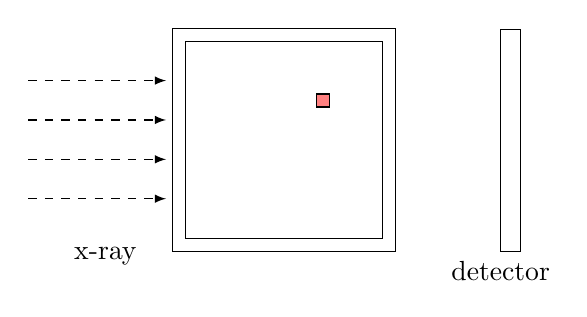
\begin{tikzpicture}[scale=0.5]

            % \draw (-6.5,2.8) rectangle (-8,2.5) node[below right, align=center] {x-ray \\ source};
            \draw (8.5,5.3) rectangle (8,-0.33) node[below] {detector};
            \draw (-0.33,-0.33) rectangle (5.33,5.33);
            \draw (0,0) rectangle (5,5);
            \draw [fill=red!50] (3.33,3.33) rectangle (3.66,3.66);
            \node [below left, xshift = -0.5cm] (-4,-1) {x-ray};
            \begin{scope} [->, >=latex]
                \foreach \i in {1,...,4}{
                    \draw[->, dashed] (-4,\i) -- (-0.5,\i);
                }
            \end{scope}
        \end{tikzpicture}
        \caption{Cross-section of x-ray}
    \end{figure}
    \begin{equation*}
        N = N_0 e^{-\mu x}
    \end{equation*}
    \begin{equation*}
        \begin{split}
            N_{h} &= N_0 \exp({ -0.6 - 0.21\cdot 10 - 0.20 - 0.21 \cdot 4 - 0.6}) = 0.013037 \cdot N_0 \\
            N_{n} &= N_0 \exp({ -0.6 - 0.21 \cdot 15 - 0.6 }) = 0.012907 \cdot N_0 
        \end{split}
    \end{equation*}

    Given that the xray has an intensity $I$ and energy $E$, then subject contrast $(C_s)$ is:
    \begin{equation}\begin{split}
        C_s &= \ln \left({\frac{I_h}{I_n}}\right) = \ln\left({ \frac{E_h }{E_n} }\right) = \ln (0.013037) - \ln(0.012907)\\
        C_s &= 0.01
    \end{split}
    \end{equation}

    Radiographic contrast($C_r$) is the product of gamma(0.5) and $C_s \implies 0.01\cdot0.5 = 0.005$.
    \subsubsection*{ii}
    \begin{figure}[h!]
        \centering
        
\begin{tikzpicture}
            [scale = 0.5]
            \fill [fill=black] (-1,-1) rectangle (6,6);
            \draw [fill=white] (-0.33,-0.33) rectangle (5.33,5.33);
            \fill [fill=gray!40] (0,0) rectangle (5,5);
            \fill [fill=gray!80] (3.33,3.33) rectangle (3.66,3.66);
        \end{tikzpicture}
        \caption{Sketch of cranial CT scan with a haemorrhage.}
    \end{figure}

\subsection*{Part B}
\subsubsection*{i}
The ratio of $T_2$ is larger than the ratio of $T_1$, suggesting that a $T_2$ weighted image would provide larger contrast between brain and blood. In order to produce this type of image, we would want $TR >> T_1$ and $TE \approx T_2$.

\subsubsection*{ii}
Contrast of zero means that the intensities would be the same, therefore:
\begin{equation*}
        92\cdot[1-\exp(-500/1500)]\cdot\exp[(-\text{TE}/60)] = 100\cdot[1-\exp(-500/2000)]\cdot\exp[(-\text{TE}/240)]
\end{equation*}

Which we solve graphically, as seen in Figure \ref{gr:IntensityxTE} and check the results using Wolframalpha: TE = \SI{13.173}{ms}.

\begin{figure}[h!]
    \centering
    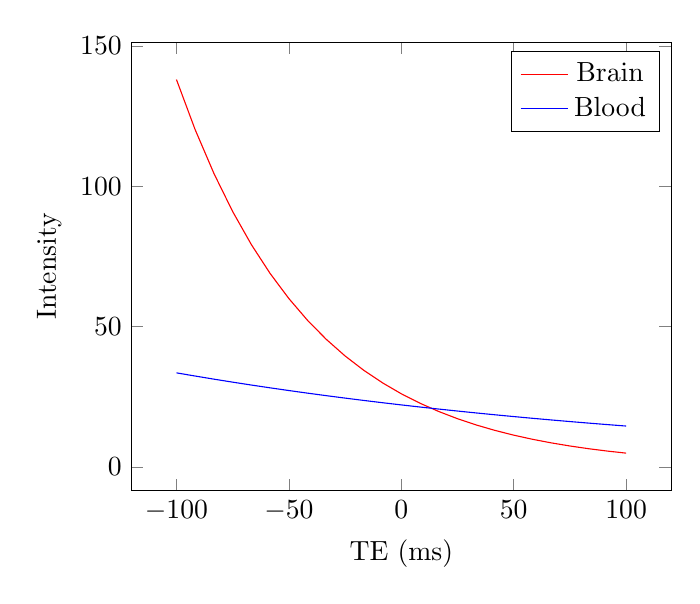
\begin{tikzpicture}
        \begin{axis} [
            domain=-100:100, xlabel=TE (ms), ylabel=Intensity,
        ]
            \addplot [red] { 92*(1-e^(-1/3))*e^(-x/60) };
            \addplot [blue] { 100*(1-e^(-1/4))*e^(-x/240) };
            \legend {Brain, Blood}
        \end{axis}
    \end{tikzpicture}
    \caption{Relationship between Intensity and TE}
    \label{gr:IntensityxTE}
\end{figure}

\subsubsection*{iii}
Using the definition of contrast ratio $(C)$ as the ratio of intensities (high/low):
\begin{equation*}\begin{split}
    I_{brain} &= 92\cdot[1-\exp(-3000/1500)]\cdot \exp(-180/60) = 3.9605 \\
    I_{blood} &= 100\cdot[1-\exp(-3000/2000)]\cdot \exp(-180/240) = 36.697 \\
    \implies C &= \frac{I_{blood}}{I_{brain}} = 9.2656
\end{split}
\end{equation*}

Alternatively we can find the Weber Contrast ($C_w$):
\begin{equation*}
    C_w = \frac{\text{high - low}}{\text{high}} = \frac{36.697 - 3.9605}{36.697} = 0.89207
\end{equation*}

\subsection*{Part C}
\subsubsection*{i}
$I_0$ is the intensity emitted by the probe, $I_{ib}$ propagates through the brain:
\begin{equation}
    \begin{split}
        \alpha = 10 \log_{10} (I_0/I) \\
        13.5 = 10 \log(0.6\cdot I_0/I_{ib}) \\
        I_{ib} = \frac{0.6 I_0}{10^{1.35}} = 0.026801 \cdot I_0 \\
    \end{split}
\end{equation}
$I_{ih}$ is incident on the haemorrhage, $I_{rh}$ is reflected by the haemorrhage:
\begin{equation}\begin{split}
    0.4 &= \log_{10} (I_{ib}/I_{ih})\\
    \implies I_{ih} &= \frac{I_{ib}}{ 10^{0.4} } = 0.010670 \cdot I_0\\
    \frac{I_{rh}}{I_{ih}} &= \frac{{(Z_2-Z_1)}^2}{{(Z_2+Z_1)}^2} = \frac{{(1.6-1.66)}^2}{{(1.6+1.66)}^2} \\
    \implies I_{rh} &= 3.3874 \times 10^{-4} \cdot I_{ih} = 3.6143 \times 10^{-6} \cdot I_0
\end{split}
\end{equation}
This is once again attenuated by brain matter, the cranium and then loses 60\% intensity ($I_r$):
\begin{equation*}
\begin{split}
    I_{r} &= 0.6 \frac{3.6143 \times 10^{-6} }{10^{0.4}\cdot 10^{1.35}} I_0 \\
    \frac{I_r}{I_0} &= 3.8563 \times 10^{-8} = -\SI{7.4138}{B}\\
    \frac{I_r}{I_0} &= -\SI{74.138}{dB} 
\end{split}
\end{equation*}
\subsubsection*{ii}
The results suggest that the intensity of the echo would be too low to form a viable image, in large part due to the attenuation of the signal through the skull (about 22 times). However, the cranium of a newborn infant brain is not yet fully fused yet, and the probe is positioned against these gaps in the cranium -- reducing this severe attenuation we experience with John's ultrasound. 